\documentclass{classrep}
\usepackage[utf8]{inputenc}
\usepackage{color}
\usepackage{amsfonts}
\usepackage{booktabs, multirow}
\usepackage{graphicx}
\usepackage{float}
\usepackage{mathtools}
\usepackage[export]{adjustbox}
\usepackage{array}


\studycycle{Informatyka, studia STACJONARNE, I st.}
\coursesemester{VI}

\coursename{Komputerowe systemy rozpoznawania}
\courseyear{2020/2021}

\courseteacher{prof. dr hab. inż. Adam Niewiadomski}
\coursegroup{Poniedziałek 13:45}

\author{
  \studentinfo{Przemysław Lis}{229940} \and
  \studentinfo{Michał Olczak}{229972} }

\title{Projekt 1. Klasyfikacja dokumentów tekstowych}

\begin{document}
\maketitle


\section{Cel projektu}
Celem projektu jest stworzenie aplikacji która podejmie się klasyfikacji 21578 artykułów prasowych z 1987 roku \cite{reuters21578}. Aplikacja odpowiedzialna będzie za sparsowanie danych i określenie jaki kraj opisuje dany artykuł. Klasyfikacja będzie możliwa w obrębie 6 klas (Kanada, USA, UK, Francja, Niemcy, Japonia) w zależności od wyżej opisanego kryterium. Do wykonania zadania wykorzystamy algorytm $k$-NN aby należycie dopasować
kraj. Oczekujemy że nasz program po analizie danych algorytmem będzie w stanie poprawnie
dopasować kraj o którym mowa lub z którego pochodzi artykuł. W projekcie porównamy również jaki wpływ na poprawność klasyfikacji oraz jej jakość będzie miało użycie różnych cech, metryk, wartości $k$ oraz odpowiedniego podziału na zbiór uczący i testowy\\
\noindent


\section{Klasyfikacja nadzorowana metodą $k$-NN}
W aplikacji wykorzystamy algorytm $k$-NN ($k$ nearest neighbours)\cite{knn1}\cite{knn2}. Jest to algorytm  regresji nieparametrycznej. Założeniem algorytmu jest że podobne problemy mają podobne rozwiązania. Algorytm sprawdza $k$ najbliższych sąsiadów (gdzie $k \in \mathbb{N}$) artykułu i w zależności od wyniku klasyfikuje jego położenie. Do obliczenia odległości artykułu od jego sąsiadów używamy różnych metryk np. Odległość Euklidesowa. Jeżeli w sąsiedztwie naszego artykułu badawczego będzie najwięcej węzłów danego typu, to wtedy zostanie on odpowiednio dopasowany do tego typu.
Parametrem wejściowym jest plik tekstowy, który następnie będzie zaklasyfikowany do odpowiedniego kraju.
Algorytm do obliczania odległości pomiędzy artykułami będzie wykorzystywał wektory cech wyekstrahowanych ($\vec{v} = \left\langle C_1, C_2, C_3, \cdots, C_n\right\rangle,\\ \, n \in [1; 10] \wedge n \in \mathbb{N}$) z artykułów (spójrz rozdział 2.1) oraz odpowiednio wybranej metryki. Algorytm jako parametry będzie przyjmował:
\vspace{5px}
\begin{enumerate*}
\setlength\itemsep{5px}
\item Wspomnianą wyżej metrykę (opisane szczegółowo w akapicie 3)
\item Zbiór artykułów których klasę znamy - zbiór uczący
\item Zbiór wyekstrahowanych cech na podstawie której odbywać się będzie klasyfikacja
\item Wartość $k$ która oznacza ile najbliższych sąsiadów będziemy brać pod uwagę przy klasyfikacji
\end{enumerate*}
\noindent

\subsection{Ekstrakcja cech, wektory cech}
1. Liczba całkowita reprezentująca największą ilość wyrazów w pierwszych 5 zdaniach.\\
\begin{displaymath}
\sum_{i = 0}^{5} s_i \textrm{, gdzie s - słowo} \wedge s \in A_{f5}\\
\end{displaymath}
Gdzie $A_{f5}$ - Fragment pierwszych 5 zdań artykułu.\\
\\
2. Stosunek liczby wystąpień słów kluczowych do długości tekstu.\\
\begin{displaymath}
\frac{\sum_{i=0}^{n}s_i}{d}\textrm{, gdzie s - słowo kluczowe, d - długość tekstu}
\end{displaymath}
3. Długość artykułu.\\
\begin{displaymath}
\sum_{i = 0}^{n} l_i \textrm{, gdzie l - litera}\\
\end{displaymath}
4. Średnia dlugość słowa.\\
\begin{displaymath}
\frac{\sum_{i=0}^{n}l_i}{\sum_{j=0}^{n}s_j}\textrm{, gdzie l - litera, s - słowo}
\end{displaymath}
5. Liczba unikalnych słów.\\
\begin{displaymath}
\sum_{i = 0}^{n} s_i \textrm{, gdzie s - słowo unikalne}\\
\end{displaymath}
%6. Liczba słów zaczynająca się dużą literą.\\
%\begin{displaymath}
%\sum_{i=0}^{n}s_i \textrm{,gdzie s - słowo zaczynające się na wielką literę}
%\end{displaymath}
6. Pierwsze wystąpienie we fragmencie tekstu nazwy kontynentu lub jego mieszkańca.\\
\begin{displaymath}
k_f = k,\, k \in C_6 \wedge k \in A
\end{displaymath}
Gdzie $k_f$ - pierwsze wystąpienie kontynentu, $k$ - kontynent ze zbioru $C_6$, \\$C_6$ - zbiór możliwych kontynentów (słów kluczowych), $A$ - artykuł
\\
\\
$C_6$ = \{Europe, European, America, American, Asia, Asian\}\\
\\
7. Liczba słów nie przekraczająca 3 znaków.\\
\begin{displaymath}
\sum_{i=0}^{n}len(s_i)<= 3 \textrm{,gdzie s - słowo}
\end{displaymath}
8. Liczba słów.\\
\begin{displaymath}
\sum_{i = 0}^{n} s_i \textrm{, gdzie s - słowo}\\
\end{displaymath}
9. Liczba słów dłuższych niż 8 znaków.\\
\begin{displaymath}
\sum_{i=0}^{n}len(s_i) > 8 \textrm{,gdzie s - słowo}
\end{displaymath}
10. Najliczniej występująca nazwa własna miasta bądź regionu ze zbioru $C_{10}$ w  pierwszych pięciu zdaniach artykułu. \\
\begin{displaymath}
%max(s_{i_1} + s_{i_1})
max\left(\sum_{i = 0}^{n} s_{i}\right), s_i \in C_{10} \wedge s_i \in A_{f5}
\end{displaymath}
Gdzie odpowiednio $s_i$ - wystąpienie regionu w tekście, $C_{10}$ -  zbiór słów kluczowych, $A_{f5}$ - Fragment pierwszych 5 zdań artykułu.\\
\\
$C_{10}$ = \{Berlin, Frankfurt, Bonn, Leverkusen, Nuremberg, Hanover, Weisbaden, 
Stuttgart, Monachium, Tokyo, Yokohama, Ottawa, Paris, Lyon, Torronto, London, Manchester, Liverpool, Birmingham, Washington, New York, Boston, Los Angeles\}
\noindent

\subsection{Miary jakości klasyfikacji} 
W naszym projekcie będziemy korzystać z 4 różnych miar jakości otrzymanej klasyfikacji (Accuracy, Precison, Recall, F1). Z pośród wymienionych 4 miar jakości, Accuracy będzie obliczana dla całego zbioru artykułów, natomiast 3 pozostałe będą obliczane zarówno dla całego zbioru artykułów jak i dla pojedynczych klas. Od tej pory będziemy korzystać również z określeń jakości przypisania klas takich jak:\\
\begin{itemize}
\item TP (True positive) - oznacza artykuły, które zostały przypisane do danej klasy i powinny do niej należeć
\item FP (False positive) - oznacza artykuły, które zostały przypisane do danej klasy i \textbf{NIE} powinny do niej należeć
\item TN (True negative) - oznacza artykuły, które \textbf{NIE} zostały przypisane do danej klasy, oraz \textbf{NIE} powinny się w niej znaleźć
\item FN (False Negative) - oznacza artykuły, które \textbf{NIE} zostały przypisane do danej klasy, ale powinny się w niej znaleźć
\end{itemize}
{\bf Accuracy} - to miara która określa dokładność klasyfikacji. Jest to stosunek ilości poprawnie zaklasyfikowanych artykułów do wszystkich artykułów. \\
Określona wzorem:
\begin{equation}\label{accuracy}
accuracy = \frac{\sum^6_{n=1} TP_n}{A}
\end{equation}

Gdzie $TP_n$ - ilość wszystkich poprawnie przypisanych artykułów do danej klasy, $A$ - liczba wszystkich artykułów
\\\\

{\bf Precision} - to miara określająca precyzję klasyfikacji elementów do danej klasy. Liczona jest tak jak accuracy, lecz w obrębie pewnej klasy.\\
Określa się wzorem:
\begin{equation}\label{precision}
precision_n = \frac{TP_n}{TP_n + FP_n}
\end{equation}

Gdzie $TP_n$ - liczba poprawnie zaklasyfikowanych artykułów do klasy $n$, $FP_n$ - liczba niepoprawnie zaklasyfikowanych artykułów do klasy $n$
\\\\
Dla całego projektu wartość precision definiowana jest jako średnia ważona precision dla danych klas:
\begin{equation}
    precision = \frac{\sum_{n=1}^{6}precision_n \cdot TP_n}{\sum_{n=1}^{6}TP_n}
\end{equation}

Gdzie $precision_n$ - wartość precyzji dla danej klasy $n$,\, $TP_n$ - artykuły poprawnie przypisane do klasy $n$.
\\\\
Miara precision przyjmuje wartości z zakresu $\langle 0, 1\rangle$ oraz należy do $\mathbb{R}$ i odpowiada za dokładność rozpoznania obiektów w obrębie danej klasy.
\\\\

{\bf Recall} - jest to miara oznaczająca odsetek poprawnie zaklasyfikowanych artykułów do danej klasy.\\
Określa się wzorem:
\begin{equation}\label{recall}
recall_n = \frac{TP_n}{TP_n + FN_n}
\end{equation}

Gdzie $TP_n$ - liczba poprawnie zaklasyfikowanych artykułów do klasy $n$, $FN_n$ - liczba artykułów które nie zostały zaklasyfikowane do klasy $n$ ale powinny się w niej znaleźć
\\\\
Dla całego projektu wartość recall definiowana jest jako średnia ważona recall dla danych klas:
\begin{equation}
    recall = \frac{\sum_{n=1}^{6}recall_n \cdot TP_n}{\sum_{n=1}^{6}TP_n}
\end{equation}

Gdzie $recall_n$ - wartość recall dla danej klasy $n$,\, $TP_n$ - artykuły poprawnie przypisane do klasy $n$.
\\\\
Miara recall przyjmuje wartości z zakresu $\langle 0, 1\rangle$ oraz należy do $\mathbb{R}$ i obrazuje stosunek poprawnie rozpoznanych artykułów do wszystkich które powinny być rozpoznane z danej klasy.
\\\\

{\bf F1} - jest to miara uśredniająca wynik. Liczona jest poprzez średnią harmoniczną precision oraz recall.\\
Określa się wzorem:
\begin{equation}\label{F1}
F1_n = 2 \cdot  \frac{precision_n \cdot recall_n}{precision_n + recall_n}
\end{equation}
\\\\
Dla całego projektu wartość F1 definiowana jest jako średnia ważona wartości F1 dla danych klas:
\begin{equation}
    F1 = \frac{\sum_{n=1}^{6}F1_n \cdot TP_n}{\sum_{n=1}^{6}TP_n}
\end{equation}

Gdzie $F1_n$ - wartość F1 dla danej klasy $n$,\, $TP_n$ - artykuły poprawnie przypisane do klasy $n$.
\\\\
Miara F1 również przyjmuje wartości z zakresu $\langle 0, 1\rangle$ oraz należy do $\mathbb{R}$.
\\\\
\begin{table}[h!]\label{tab_classification_example}
\centering
\begin{tabular}{cc|cccccc|}
\cline{3-8}
 &  & \multicolumn{6}{c|}{\textbf{Rzeczywista Klasa Artykułu}} \\ \cline{3-8} 
 &  & \multicolumn{1}{c|}{\textbf{USA}} & \multicolumn{1}{c|}{\textbf{UK}} & \multicolumn{1}{c|}{\textbf{Canada}} & \multicolumn{1}{c|}{\textbf{Germany}} & \multicolumn{1}{c|}{\textbf{France}} & \textbf{Japan} \\ \hline
\multicolumn{1}{|c|}{\multirow{6}{*}{\textbf{\begin{tabular}[c]{@{}c@{}}Dopaso-\\wana\\ Klasa\\ Artykułu\end{tabular}}}} & \textbf{Usa} & \multicolumn{1}{c|}{5411} & \multicolumn{1}{c|}{114} & \multicolumn{1}{c|}{96} & \multicolumn{1}{c|}{65} & \multicolumn{1}{c|}{41} & 23 \\ \cline{2-8} 
\multicolumn{1}{|c|}{} & \textbf{UK} & \multicolumn{1}{c|}{354} & \multicolumn{1}{c|}{3790} & \multicolumn{1}{c|}{222} & \multicolumn{1}{c|}{142} & \multicolumn{1}{c|}{75} & 9 \\ \cline{2-8} 
\multicolumn{1}{|c|}{} & \textbf{Canada} & \multicolumn{1}{c|}{311} & \multicolumn{1}{c|}{120} & \multicolumn{1}{c|}{2255} & \multicolumn{1}{c|}{105} & \multicolumn{1}{c|}{45} & 29 \\ \cline{2-8} 
\multicolumn{1}{|c|}{} & \textbf{Germany} & \multicolumn{1}{c|}{123} & \multicolumn{1}{c|}{91} & \multicolumn{1}{c|}{18} & \multicolumn{1}{c|}{1725} & \multicolumn{1}{c|}{135} & 17 \\ \cline{2-8} 
\multicolumn{1}{|c|}{} & \textbf{France} & \multicolumn{1}{c|}{100} & \multicolumn{1}{c|}{75} & \multicolumn{1}{c|}{66} & \multicolumn{1}{c|}{25} & \multicolumn{1}{c|}{1510} & 9 \\ \cline{2-8} 
\multicolumn{1}{|c|}{} & \textbf{Japan} & \multicolumn{1}{c|}{18} & \multicolumn{1}{c|}{14} & \multicolumn{1}{c|}{52} & \multicolumn{1}{c|}{17} & \multicolumn{1}{c|}{7} & 312 \\ \hline
\end{tabular}
\caption{Przykładowy wynik klasyfikacji}
\end{table}
\\\\
Na podstawie powyższej tabeli oraz wzorów \ref{accuracy}, \ref{precision}, \ref{recall}, \ref{F1} obliczamy wartości miar końcowych dla przykładowych wartości klasyfikacji.
\\\\
\begin{table}[H]\label{tab_quality_example}
\centering
\begin{tabular}{c|c|c|c|c|}
\cline{2-5}
 & Precision & Recall & F1 & Accuracy \\ \hline
\multicolumn{1}{|c|}{USA} & 0.9410 & 0.8566 & 0.9419 & \multirow{7}{*}{0.8563} \\ \cline{1-4}
\multicolumn{1}{|c|}{UK} & 0.8253 & 0.9015 & 0.8242 &  \\ \cline{1-4}
\multicolumn{1}{|c|}{Canada} & 0.7871 & 0.8324 & 0.7886 &  \\ \cline{1-4}
\multicolumn{1}{|c|}{Germany} & 0.8179 & 0.8297 & 0.8254 &  \\ \cline{1-4}
\multicolumn{1}{|c|}{France} & 0.8459 & 0.8329 & 0.8503 &  \\ \cline{1-4}
\multicolumn{1}{|c|}{Japan} & 0.7486 & 0.7666 & 0.7533 &  \\ \cline{1-4}
\multicolumn{1}{|c|}{Średnia} & 0.8276 & 0.8366 & 0.8306 &  \\ \cline{1-5} 
\end{tabular}
\caption{Przykładowe wartości miar obliczone na podstawie tabeli \ref{tab_classification_example}}
\end{table}

\section{Klasyfikacja z użyciem metryk i miar podobieństwa tekstów}


W naszym projekcie do obliczenia odległośi danych artykułów wykorzystaliśmy trzy metryki:

\def\engram_foot{W przypadku cech liczbowych jest to różnica ich wartości, w przypadku cech tekstowych obliczany jest 1-$sim_n$ (patrz wzór \ref{ngram})}

\begin{itemize}
  \item Metryka Euklidesowa - Aby obliczyć odległość $d_e$ między dwoma artykułami $X, Y$ należy obliczyć pierwiastek sumy kwadratów odległości wartości cech o tych samych indeksach.
    \begin{equation}\label{euklides}
        d_e(X,Y) = \sqrt{\sum_{i=1}^{n}(x_i - y_i)^2}
    \end{equation}
    Gdzie $d_e$ - odległość euklidesowa, $X, Y$ - wektory cech artykułów pomiędzy którymi liczymy odległość, $x_i, y_i$ - wartości cech wektorów ($X, Y$)\footnote{\engram_foot}\\\
    
  \item Metryka Manhattan (miejska) - Aby obliczyć odległość $d_m$ między dwoma artykułami $X, Y$ należy obliczyć sumę wartości bezwzględnych odległości poszczególnych cech $x_i, y_i$
    \begin{equation}\label{manhattan}
        d_{m}(X,Y) = \sum_{i=1}^{n} | x_i - y_i |
    \end{equation}
    gdzie: $d_m$ - odległość miejska, $X, Y$ - wektory cech artykułów pomiędzy którymi liczymy odległość, $x_i, y_i$ - wartości cech wektorów ($X, Y$)\footnotemark[\value{footnote}]\\
    
  \item Metryka Czebyszewa - Aby obliczyć odległość $d_{Ch}$ między dwoma artykułamu $X, Y$ należy wybrać maksymalną wartość, wartości bezwzględnych odległości pomiędzy poszczególnymi wartościami cech $x_i, y_i$
    \begin{equation}\label{czebyszew}
        d_{Ch}(X,Y)= \max_{i}{|x_i - y_i|}
    \end{equation}
    gdzie: $d_{Ch}$ - odległość Czebyszewa, $X, Y$ - wektory cech artykułów pomiędzy którymi liczymy odległość, $x_i, y_i$ - wartości cech wektorów ($X, Y$)\footnotemark[\value{footnote}]\\
\end{itemize}

Aby obliczyć podobieństwo łańcuchów tekstowych zastosowaliśmy miarę $n$-gramów. Metoda ta opiera się na sprawdzaniu podobieństwa dwóch łańcuchów tekstowych na podstawie ilości wspólnych podciągów w łańcuchach $s_1$ oraz $s_2$. Jako $s_1$ zawsze przyjmujemy krótsze z dwóch słów. Jeżeli krótsze słowo ma więcej niż 3 litery to przyjmujemy $n$ = 3, w przeciwnym przypadku n jest równe długości krótszego słowa. Miara ta przyjmuje wartości z zakresu $\langle 0, 1\rangle$ oraz należy do $\mathbb{R}$.

\begin{equation}\label{ngram}
        sim_n(s_1,s_2) = \frac{1}{N-n+1} \sum_{i=1}^{N-n+1}h(i)
\end{equation}

gdzie, $sim_n$ - wartość prawdopodobieństwa $h(i)$ - funkcja zwracającaa wartość 1 jeżeli ciąg z $s_1$ występuje przynajmniej raz w $s_2$ w przeciwnym wypadku funkcja zwraca wartość 0, $N-n+1$ - ilość możliwych $n$-elementowych podciągów w $s_1$\\

Aby obliczyć odległość pomiędzy dwoma wartościami tekstowymi musimy najpierw obliczyć podobieństwo pomiędzy tymi tekstami (wzór \ref{ngram} i następnie odjąć je od 1:
\begin{equation}\label{tekstDist}
        d(s_1,s_2) = 1 - sim_n(s_1,s_2)
\end{equation}
gdzie: $d$ - odległość pomiędzy dwoma cechami tekstowymi, $s_1, s_2$ - wartości tekstowe cech, $sim_n$ - podobieństwo pomiędzy dwoma wartościami tekstowymi (wzór \ref{ngram}).\\\\
Przykładowo dla $s_1$ = "kaptur" i $s_2$ = "kapelusz" mamy $n = 3$ i:
\begin{equation}\label{dsimExample}
    d(s1, s2) = 1 - \frac{1}{4} \cdot (1 + 0 + 0 + 0) = 1 - \frac{1}{4} = \frac{3}{4}
\end{equation}

\newpage

Przyjmijmy przykładowe wektory:\\
\begin{enumerate}
    \item X = ["Boston", "", "America", "Statue of Liberty", "", "Inc", "White House", "United States", 0, 7, 1, 5, 24, 234, 12]
    \item Y = ["New York", "", "Canada", "Europe", "kilograms", "Inc", \\"Germany", "Berlin Wall", 14, 2, 4, 4, 0, 200, 110]
\end{enumerate}\leavevmode\newline

Dla podanych wektorów otrzymujemy:\\
\begin{itemize}
    \item Metryka \textbf{Euklidesowa}
    \begin{equation}\label{euklidesExample}
    \begin{multlined}
        d_e(X,Y) = (1^2+0^2+1^2+1^2+1^2+0^2+1^2+1^2\\
        \shoveleft +14^2+5^2+3^2+1^2+24^2+34^2+98^2)^\frac{1}{2}=\\
        \shoveleft = \sqrt{1+0+1+1+1+0+1+1+196+25+9+1+576+1156+9604}\\= 107.58
    \end{multlined}
    \end{equation}
    \item Metryka \textbf{Manhattan}
    \begin{equation}\label{taxiExample}
    \begin{multlined}
        d_m(X,Y) = |1-0|+|1-1|+|1-0|+|1-0|+|1-0|+|1-1|\\
        \shoveleft +|1-0|+|1-0|+|0-14|+|7-2|+|1-4|+|5-4|\\
        \shoveleft +|24-0|+|234-200|+|12-110| = 1+0+1+1+1+0\\
        \shoveleft +1+1+14+5+3+1+24+34+98 = 185
    \end{multlined}
    \end{equation}
    \item Metryka \textbf{Czebyszewa}:
    \begin{equation}\label{czebyszewExample}
    \begin{multlined}
        d_{Ch}(X,Y) = \max(|1|, |0|, |1|, |1|, |1|,|0|,\\
        \shoveleft |1|, |1|, |14|, |5|, |3|, |1|, |24|, |34|, |98|) = 98
    \end{multlined}
    \end{equation}
\end{itemize}


\section{Budowa aplikacji}
\subsection{Diagramy UML}

\begin{figure}[!htbp]
	\centering
     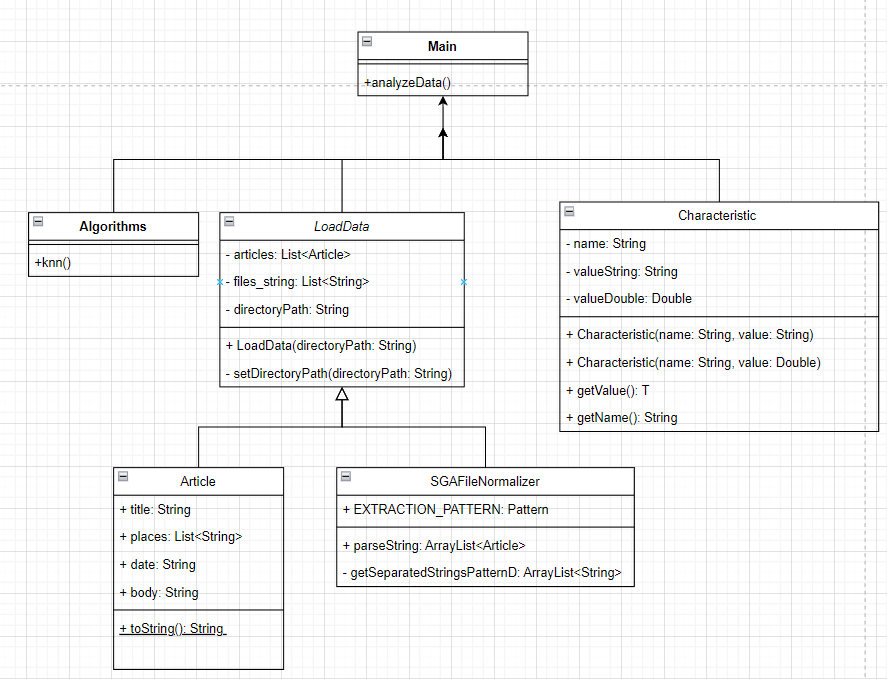
\includegraphics[width=\textwidth]{img/uml.png}
	\caption{Diagram UML projektu}
\end{figure}
\vspace{5px}
\noindent - {\bf Klasa Main}\\
Program posiada klasę Main której zadaniem jest obsługa całego algorytmu. funkcją tej klasy jest kontrolowanie wczytania danych jak i obsługa algorytmu jak i użycia charakterystyk. Klasa ta jako rezulatat będzie zwracać wyniki metryk dla danych wartości algorytmu.\\\\
- {\bf Klasa Algorithms}\\
W tej klasie będzie przechowywany algorytm KNN. Cała implementacja tego algorytmu będzie miała swoje miejsce w tej klasie.\\\\
- {\bf Klasa LoadData}\\
Kolejną klasą jest LoadData która będzie służyła do ładowania plików. Aby poprawnie to zrobić będą potrzebne kolejne klasy takie jak {\bf Article} która przechowuje informacje na temat artykułu. Posiada ona atrybuty takie jak tytuł, miejsce, date oraz treść artykułu. Klasa ta posiada metodę toString aby zwrócić wszystkie dane odnośnie artykułu. Kolejną klasą która będzie potrzebna w poprawnym ładowaniu danych jest {\bf SGAFileNormalizer} która w swoich atrybutach posiada definicje typu regex która pomoże wyekstrachować dane z dokumentu w taki sposób jaki jest nam potrzebny do poprawnego działania algorytmu.\\\\
- {\bf Klasa Characteristic}\\
Jest to klasa która będzie generycznie tworzona w oparciu o charakterystyki z punktu 2.1. Głównym zadaniem tej klasy będzie przechowywanie danych oraz algorytmów potrzebnych do obliczania macierz charakterystyk.


\subsection{Prezentacja wyników, interfejs użytkownika} 
Krótki ilustrowany opis jak użytkownik może korzystać z aplikacji, w~szczególności wprowadzać parametry klasyfikacji i odczytywać wyniki. Wersja JRE i inne wymogi
niezbędne do uruchomienia aplikacji przez użytkownika na własnym komputerze. \\
\noindent {\bf Sekcja uzupełniona jako efekt zadania Tydzień 05 wg Harmonogramu Zajęć
na WIKAMP KSR.}

\section{Wyniki klasyfikacji dla różnych parametrów wejściowych}
Wstępne wyniki miary Accuracy dla próbnych klasyfikacji na ograniczonym zbiorze tekstów (podać parametry i kryteria
wyboru wg punktów 3.-8. z opisu Projektu 1.). 
\noindent {\bf Sekcja uzupełniona jako efekt zadania Tydzień 05 wg Harmonogramu Zajęć
na WIKAMP KSR.}


\section{Dyskusja, wnioski, sprawozdanie końcowe}

Wyniki kolejnych eksperymentów wg punktów 2.-8. opisu projektu 1.  Wykresy i tabele
obowiązkowe, dokładnie opisane w ,,captions'' (tytułach), konieczny opis osi i
jednostek wykresów oraz kolumn i wierszy tabel.\\ 

{**Ewentualne wyniki realizacji punktu 9. opisu Projektu 1., czyli,,na ocenę 5.0'' i ich porównanie do wyników z
części obowiązkowej**.Dokładne interpretacje uzyskanych wyników w zależności od parametrów klasyfikacji
opisanych w punktach 3.-8 opisu Projektu 1. 
Szczególnie istotne są wnioski o charakterze uniwersalnym, istotne dla podobnych zadań. 
Omówić i wyjaśnić napotkane problemy (jeśli były). Każdy wniosek/problem powinien mieć poparcie
w przeprowadzonych eksperymentach (odwołania do konkretnych wyników: wykresów,
tabel). \\
\underline{Dla końcowej oceny jest to najważniejsza sekcja} sprawozdania, gdyż prezentuje poziom
zrozumienia rozwiązywanego problemu.\\

** Możliwości kontynuacji prac w obszarze systemów rozpoznawania, zwłaszcza w kontekście pracy inżynierskiej,
magisterskiej, naukowej, itp. **\\

\noindent {\bf Sekcja uzupełniona jako efekt zadania Tydzień 06 wg Harmonogramu Zajęć
na WIKAMP KSR.}


\section{Braki w realizacji projektu 1.}
Wymienić wg opisu Projektu 1. wszystkie niezrealizowane obowiązkowe elementy projektu, ewentualnie
podać merytoryczne (ale nie czasowe) przyczyny tych braków. 


\begin{thebibliography}{0}
\bibitem{reuters21578} Zbiór 21578 sklasyfikowanych tekstów. \url{http://archive.ics.uci.edu/ml/
datasets/Reuters-21578+Text+Categorization+Collection}
\bibitem{knn1} \url{https://www.nature.com/articles/s41598-022-10358-x}
\bibitem{knn2} Materiał wideo objaśniający algorytm $k$-nn. \url{https://www.youtube.com/watch?v=IPqZKn_cMts}
\bibitem{tadeusiewicz90} R. Tadeusiewicz: Rozpoznawanie obrazów, PWN, Warszawa, 1991.  
\bibitem{niewiadomski08} A. Niewiadomski, Methods for the Linguistic Summarization of Data: Applications of Fuzzy Sets and Their Extensions, Akademicka Oficyna Wydawnicza EXIT, Warszawa, 2008.
\end{thebibliography}

Literatura zawiera wyłącznie źródła recenzowane i/lub o potwierdzonej wiarygodności,
możliwe do weryfikacji i cytowane w sprawozdaniu. 
\end{document}
